\chapter{Aufbau eines reduzierten Reaktormodells}
    Ziel der Konstruktion eines reduzierten Reaktormodells (Reduced-Order-Model, ROM) ist es, durch Kombination mehrerer idealer Reaktoren ein Reaktornetzwerk aufzubauen, das eine möglichst genaue Modellierung des Reaktors ermöglicht. Dabei werden Strömungserscheinungen wie Bypass, Rezirkulation oder Reformierungszone. durch einzelne Reaktoren abgebildet. 
\iffalse
    \section{Rahmenbedingungen}
        Grundlage der Simulation ist ein Reaktor, an dem bereits experimentell zwei Versuche durchgeführt wurden, bei denen die Temperaturen und Stoffströme am Reaktorausgang ermittelt wurden. Die Rahmenbedingungen beider Versuche sind in Tabelle \ref{tab:rahmenbedingungen_versuche} dargestellt.
        \begin{table}[H]
            \centering
            \caption{Vergleich der Prozessfälle \cite{gonzales}}
            \begin{tabular}{llll}
            \toprule
            \textbf{Variablen} & & \textbf{Fall 1} & \textbf{Fall 2} \\
            \midrule
            \textbf{1. Erdgas} & Temperatur [°C] & 66,6 & 67,5 \\
                               & Massenstrom [kg/h] & 182,4 & 153,3 \\
            \midrule
            \textbf{2. Kohlendioxid} & Temperatur [°C] & -- & 67,5 \\
                                     & Massenstrom [kg/h] & 0 & 196,4 \\
            \midrule
            \textbf{3. Sauerstoff} & Temperatur [°C] & 231,9 & 231,2 \\
                                   & Massenstrom [kg/h] & 252,2 & 246,9 \\
            \midrule
            \textbf{4. Dampf} & Temperatur [°C] & 353,4 & 353,4 \\
                              & Massenstrom [kg/h] & 38,7 & 39,4 \\
            \midrule
            Wandwärmeverlust [kW] & & 30 & 30 \\
            Reaktorvolumen [L] & & 134 & 134 \\
            \midrule
            \textbf{Kommentar} & & Referenz & CO\textsubscript{2}-Zugabe \\
            \bottomrule
            \end{tabular}
            \label{tab:rahmenbedingungen_versuche}
        \end{table}
        Neben den Werten des Feedstroms sind zusätzlich die Geometrien des Reaktors und des Brenners bekannt, die in Abbildung \ref{fig:reaktorgeometrie} dargestellt sind. 
        \begin{figure}[H]
            \centering
            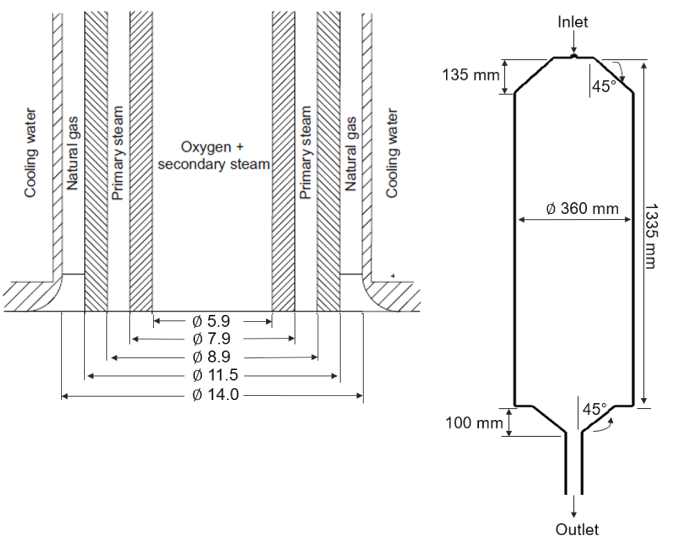
\includegraphics[width=0.8\linewidth]{img/sonstiges/Reaktorgeometrien.png}
            \caption{Geometrien des Reaktors sowie des Brenners}
            \label{fig:reaktorgeometrie}
        \end{figure}
    \section{Vorbetrachtungen}
        Zur Vorbetrachtung liegt bereits eine CFD-Analyse sowie ein komplexes ROM-Modell vor. 
        \begin{figure}[H]
            \centering
            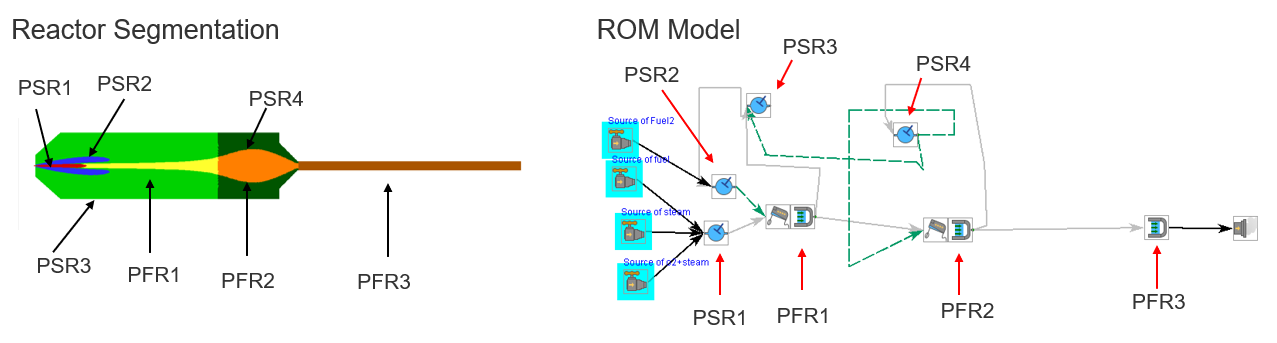
\includegraphics[width=1\linewidth]{img/sonstiges/Reactor Segmentation.png}
            \caption{Reaktorsegmentierung und komplexes ROM auf basis einer CFD-Simulation \cite{gonzales}}
            \label{fig:reaktorsegmentierung}
        \end{figure}
        Um den Einfluss der einzelnen Reaktoren auf die Simulationsergebnisse zu ermitteln, wird das in Abschnitt \ref{sec:Simulationen_reaktionsmechanismus} dargestellte Reaktornetzwerk schrittweise erweitert. Nach jeder Erweiterung werden die Simulationsergebnisse mit den Experimentaldaten verglichen. 

        Durch diesen iterativen Ansatz lässt sich nicht nur die Relevanz einzelner Reaktoren für die Abbildung der experimentellen Daten bestimmen, sondern auch eine Grundlage für die spätere Modellvereinfachung schaffen. Auf diese Weise kann zwischen einer möglichst hohen Modellgenauigkeit und einer zugleich geringen Rechenkomplexität abgewogen werden. Zudem wird sichtbar, welche Teilreaktoren für die wesentlichen Stoff- und Energiebilanzen entscheidend sind und welche nur einen geringen Beitrag zur Gesamtvorhersage leisten. Damit wird eine systematische Basis geschaffen, um in späteren Schritten reduzierte Modelle (ROMs) abzuleiten, die für Prozessoptimierungen und Echtzeitanwendungen besser geeignet sind.
\fi 
    \section*{Entwicklung eines komplexen Reaktornetzwerks}
        \label{sec:erweiterung_rom}
        Im Folgenden werden die einzelnen Entwicklungsschritte eines einfachen Modells, wie es bereits beschrieben wurde, bis zu einem komplexen Netzwerk einzeln aufgeführt. Dabei sind die Reaktoren, welche die Flamm- sowie Bypasszone darstellen, orange gefärbt, während die Reaktoren der Reformierungszone blau dargestellt sind. Die ab Reaktornetzwerk 3 verwendete Rezirkulationszone bzw. die Rezirkulationszonen sind zusätzlich grün dargestellt.
        \subsection*{Reaktornetzwerk 1}
            Abbildung \ref{fig:reaktornetzwerk1} zeigt die einfachste Form des untersuchten Reaktornetzwerks, bestehend aus einem PSR und einem nachgeschalteten PFR. In diesem Aufbau wird zunächst die schnelle chemische Umsetzung im PSR angenommen, der durch vollständige Durchmischung charakterisiert ist. Anschließend erfolgt im PFR eine strömungsdominierte Nachreaktion, in der axiale Temperatur- und Konzentrationsverläufe berücksichtigt werden. Der Wärmeverlust erfolgt ausschließlich über den PFR.

            Dieses zweistufige Modell ist die Grundlage für alle folgenden Erweiterungen und ermöglicht eine erste Beschreibung der Hauptreaktionen während der partiellen Oxidation.
            \begin{figure}[H]
                \centering
                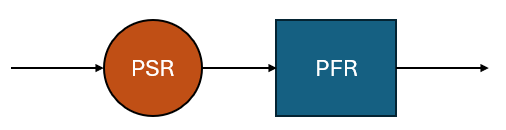
\includegraphics[width=0.7\linewidth]{img/Erweiterungen/1.png}
                \caption{Schematische Darstellung des ersten Reaktornetzwerks, bestehend aus einer Flammzone (orange) und einer Nachbrennzone (blau)}
                \label{fig:reaktornetzwerk1}
            \end{figure}
            Dabei hat der PSR ein Volumen von 13,7~Litern, während der PFR ein Volumen von ca. 116~Litern aufweist. Insgesamt ergibt sich so das in Tabelle \ref{tab:rahmenbedingungen_versuche} beschriebene Volumen von 130 Litern. Der Wärmeverlust wird vollständig durch den PFR abgebildet und beträgt 30~kW. 
        \subsection*{Reaktornetzwerk 2}
            Im nächsten Schritt (Abbildung \ref{fig:reaktornetzwerk2}) wird das System um einen zweiten PSR erweitert, der die Einspeisung eines zweiten Stoffstroms parallel zur Flammzone ermöglicht. 

            Diese Konfiguration dient der realitätsnäheren Beschreibung des Zulaufs, da ein Teil des eingebrachten Erdgases an der Flammzone vorbeiströmt (Bypass). Durch diese Erweiterung liegt am PFR-Eintritt eine veränderte Gaszusammensetzung vor. In diesem PSR befindet sich ausschließlich Erdgas, da dieses als äußeres Feedgas (siehe Abbildung \ref{fig:reaktorgeometrie}) zugeführt wird. Im Vergleich zum vorhergehenden Reaktornetzwerk wurde der Erdgasstrom zu gleichen Verhältnissen aufgeteilt, die sonstigen Stoffströme verlaufen vollständig durch den PSR, der die Flammzone darstellt.  
            \begin{figure}[H]
                \centering
                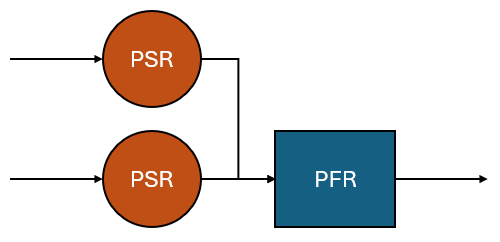
\includegraphics[width=0.7\linewidth]{img/Erweiterungen/2.png}
                \caption{Schematische Darstellung des zweiten Reaktornetzwerks, bestehend aus Flammzone mit Bypass (orange) und einer Nachbrennzone (blau)}
                \label{fig:reaktornetzwerk2}
            \end{figure}
        \subsection*{Reaktornetzwerk 3}
            Das Reaktornetzwerk 2 wird um eine Rezirkulationszone erweitert. Um einen Stoffaustausch zwischen dem PFR und der Rezirkulationszone zu ermöglichen, wird der PFR in mehrere PFRs unterteilt. In diesem vereinfachten Modell wird davon ausgegangen, dass die Rezirkulationszone nur im Austausch mit dem Ende des Reaktors und der Bypass Zone steht. Es wird ein zusätzlicher PFR als Reaktorausgang hinzugefügt. Im Bereich des ersten PFRs tritt kein Wärmeverluststrom auf, da dieser am PSR, der die Rezirkulationszone darstellt, simuliert wird. Der Gesamtwärmeverluststrom ergibt sich insgesamt aus dem Wärmeverluststrom des PSRs der Rezirkulationszone (20~kW) und dem Wärmeverluststrom des zweiten PFRs (10~kW). 

            Das Rezirkulationsverhältnis wurde auf 0,95 festgelegt. Damit wird ein sehr hoher Anteil des Abgasstroms aus der Nachbrennzone erneut in das Reaktorsystem zurückgeführt. Konkret bedeutet dies, dass 95~\% des aus der Nachbrennzone austretenden Massenstroms rezirkuliert und nur 5~\% als Produktstrom abgeführt werden. 
            \begin{figure}[H]
                \centering
                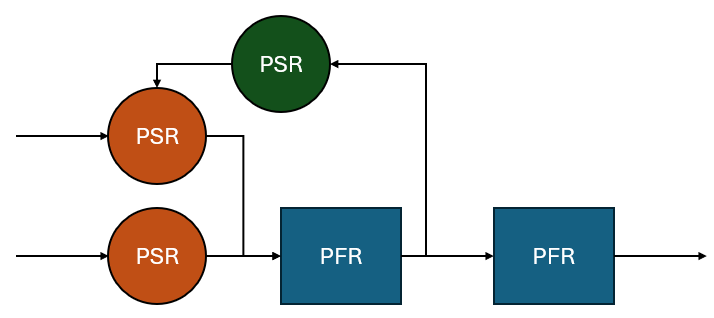
\includegraphics[width=0.8\linewidth]{img/Erweiterungen/3.png}
                \caption{Schematische Darstellung des dritten Reaktornetzwerks, bestehend aus Flammzone mit Bypass (orange), einer Nachbrennzone (blau) und einer Rezirkulationszone (grün)}
                \label{fig:reaktornetzwerk3}
            \end{figure}
            In diesem Modell ist der Durchmesser und die Länge des ersten PFRs sehr gering, weshalb die Rezirkulationszone einen großen Anteil am Volumen einnimmt. 
        \subsection*{Reaktornetzwerk 4}
            Im Vergleich zum vorherigen Reaktornetzwerk wurde ein Stoffstrom von der Mitte des ursprünglichen PFRs zur Rezirkulationszone hinzugefügt, sodass diese jetzt mit mehreren Reaktoren gekoppelt ist. Dies ist in Abbildung \ref{fig:reaktornetzwerk4} dargestellt. Dieses Rezirkulations\-verhältnis wurde analog zu Reaktornetzwerk 3 als 0,95 festgelegt. Die Wärmeverlustströme sind wie in Modell 3 definiert. 
            \begin{figure}[H]
                \centering
                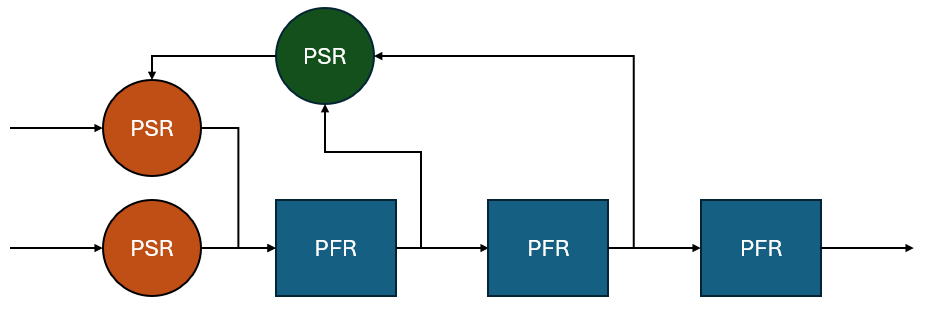
\includegraphics[width=0.8\linewidth]{img/Erweiterungen/4.png}
                \caption{Schematische Darstellung des vierten Reaktornetzwerks, bestehend aus Flammzone mit Bypass (orange), einer Nachbrennzone (blau) und einer Rezirkulationszone (grün)}
                \label{fig:reaktornetzwerk4}
            \end{figure}
        \subsection*{Reaktornetzwerk 5}
            Im finalen Schritt wird die Rezirkulationszone in zwei verschiedene Reaktoren unterteilt und es werden Stoffströme von beiden Reaktoren in der Rezirkulationszone zur Nachbrennzone berücksichtigt. Der linke PSR umfasst etwa 75~\% und der rechte PSR etwa 25~\% des ursprünglichen Volumens der Rezirkulationszone. Das Reaktornetzwerk ist in Abbildung \ref{fig:reaktornetzwerk5} dargestellt. Die Wärmeverluste der in Netzwerk 3 beschriebenen Rezirkulationszone werden abhängig von den Volumina auf beide PSRs aufgeteilt. Die Auftrennung der Stoffströme nach den Reaktoren der Rezirkulationszone entsprechen 0,5.
            \begin{figure}[H]
                \centering
                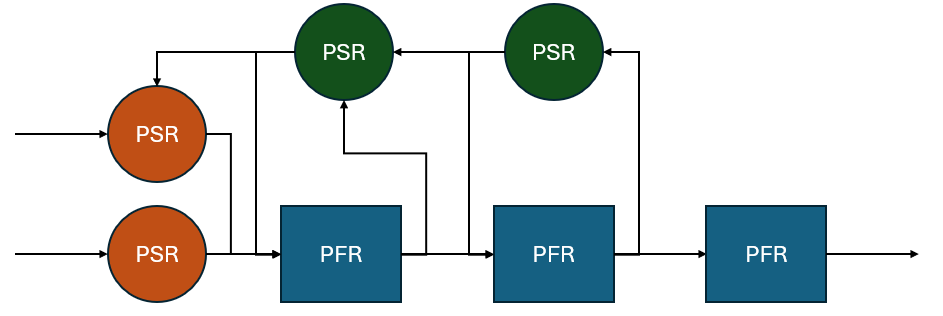
\includegraphics[width=0.8\linewidth]{img/Erweiterungen/5.png}
                \caption{Schematische Darstellung des fünften Reaktornetzwerks, bestehend aus Flammzone mit Bypass (orange), einer Nachbrennzone (blau) und einer Rezirkulationszone aus zwei PSRs (grün)}
                \label{fig:reaktornetzwerk5}
            \end{figure}
\iffalse
    \section{Auswertung}
        \iffalse
        Da sich in den oben beschriebenen Reaktionsmechanismen die Länge der PFRs unterscheidet, ist ein direkter Vergleich der Verläufe innerhalb dieser Reaktoren nicht umsetzbar. Vergleichbar sind jedoch einzelne Punkte im Reaktor sowie die Zusammensetzung und Temperatur des Gases am Outlet. In Abbildung \ref{fig:erweiterungen_messpunkte} ist dargestellt, um welche Messpunkte es sich handelt. 
        \begin{figure}[H]
            \centering
            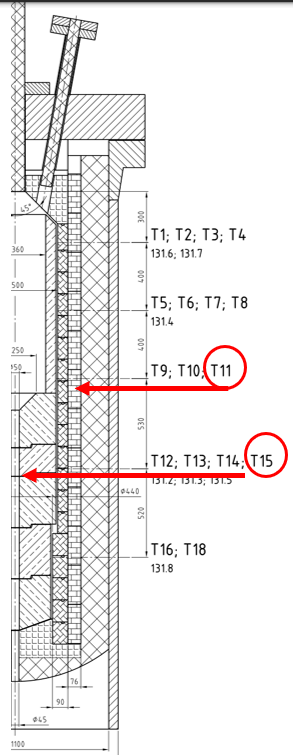
\includegraphics[width=0.2\linewidth]{img/Erweiterungen/Messpunkte.png}
            \caption{Messpunkte im Reaktor \cite{gonzales}}
            \label{fig:erweiterungen_messpunkte}
        \end{figure}
        \fi 

        Da sich in den oben beschriebenen Reaktionsmechanismen die Länge der PFRs unterscheidet, ist ein direkter Vergleich der Verläufe innerhalb dieser Reaktoren nicht umsetzbar. Vergleichbar sind allerdings die Zusammensetzungen der Gase am Outlet, zu denen auch Experimentelle Daten zum Vergleich vorliegen. In Abbildung \ref{fig:erweiterungen_vergleich_stoffe} sind die ermittelten Gaszusammensetzungen im Vergleich zu den Experimentell ermittelten Werten dargestellt. 
        \begin{figure}[H]
            \centering
            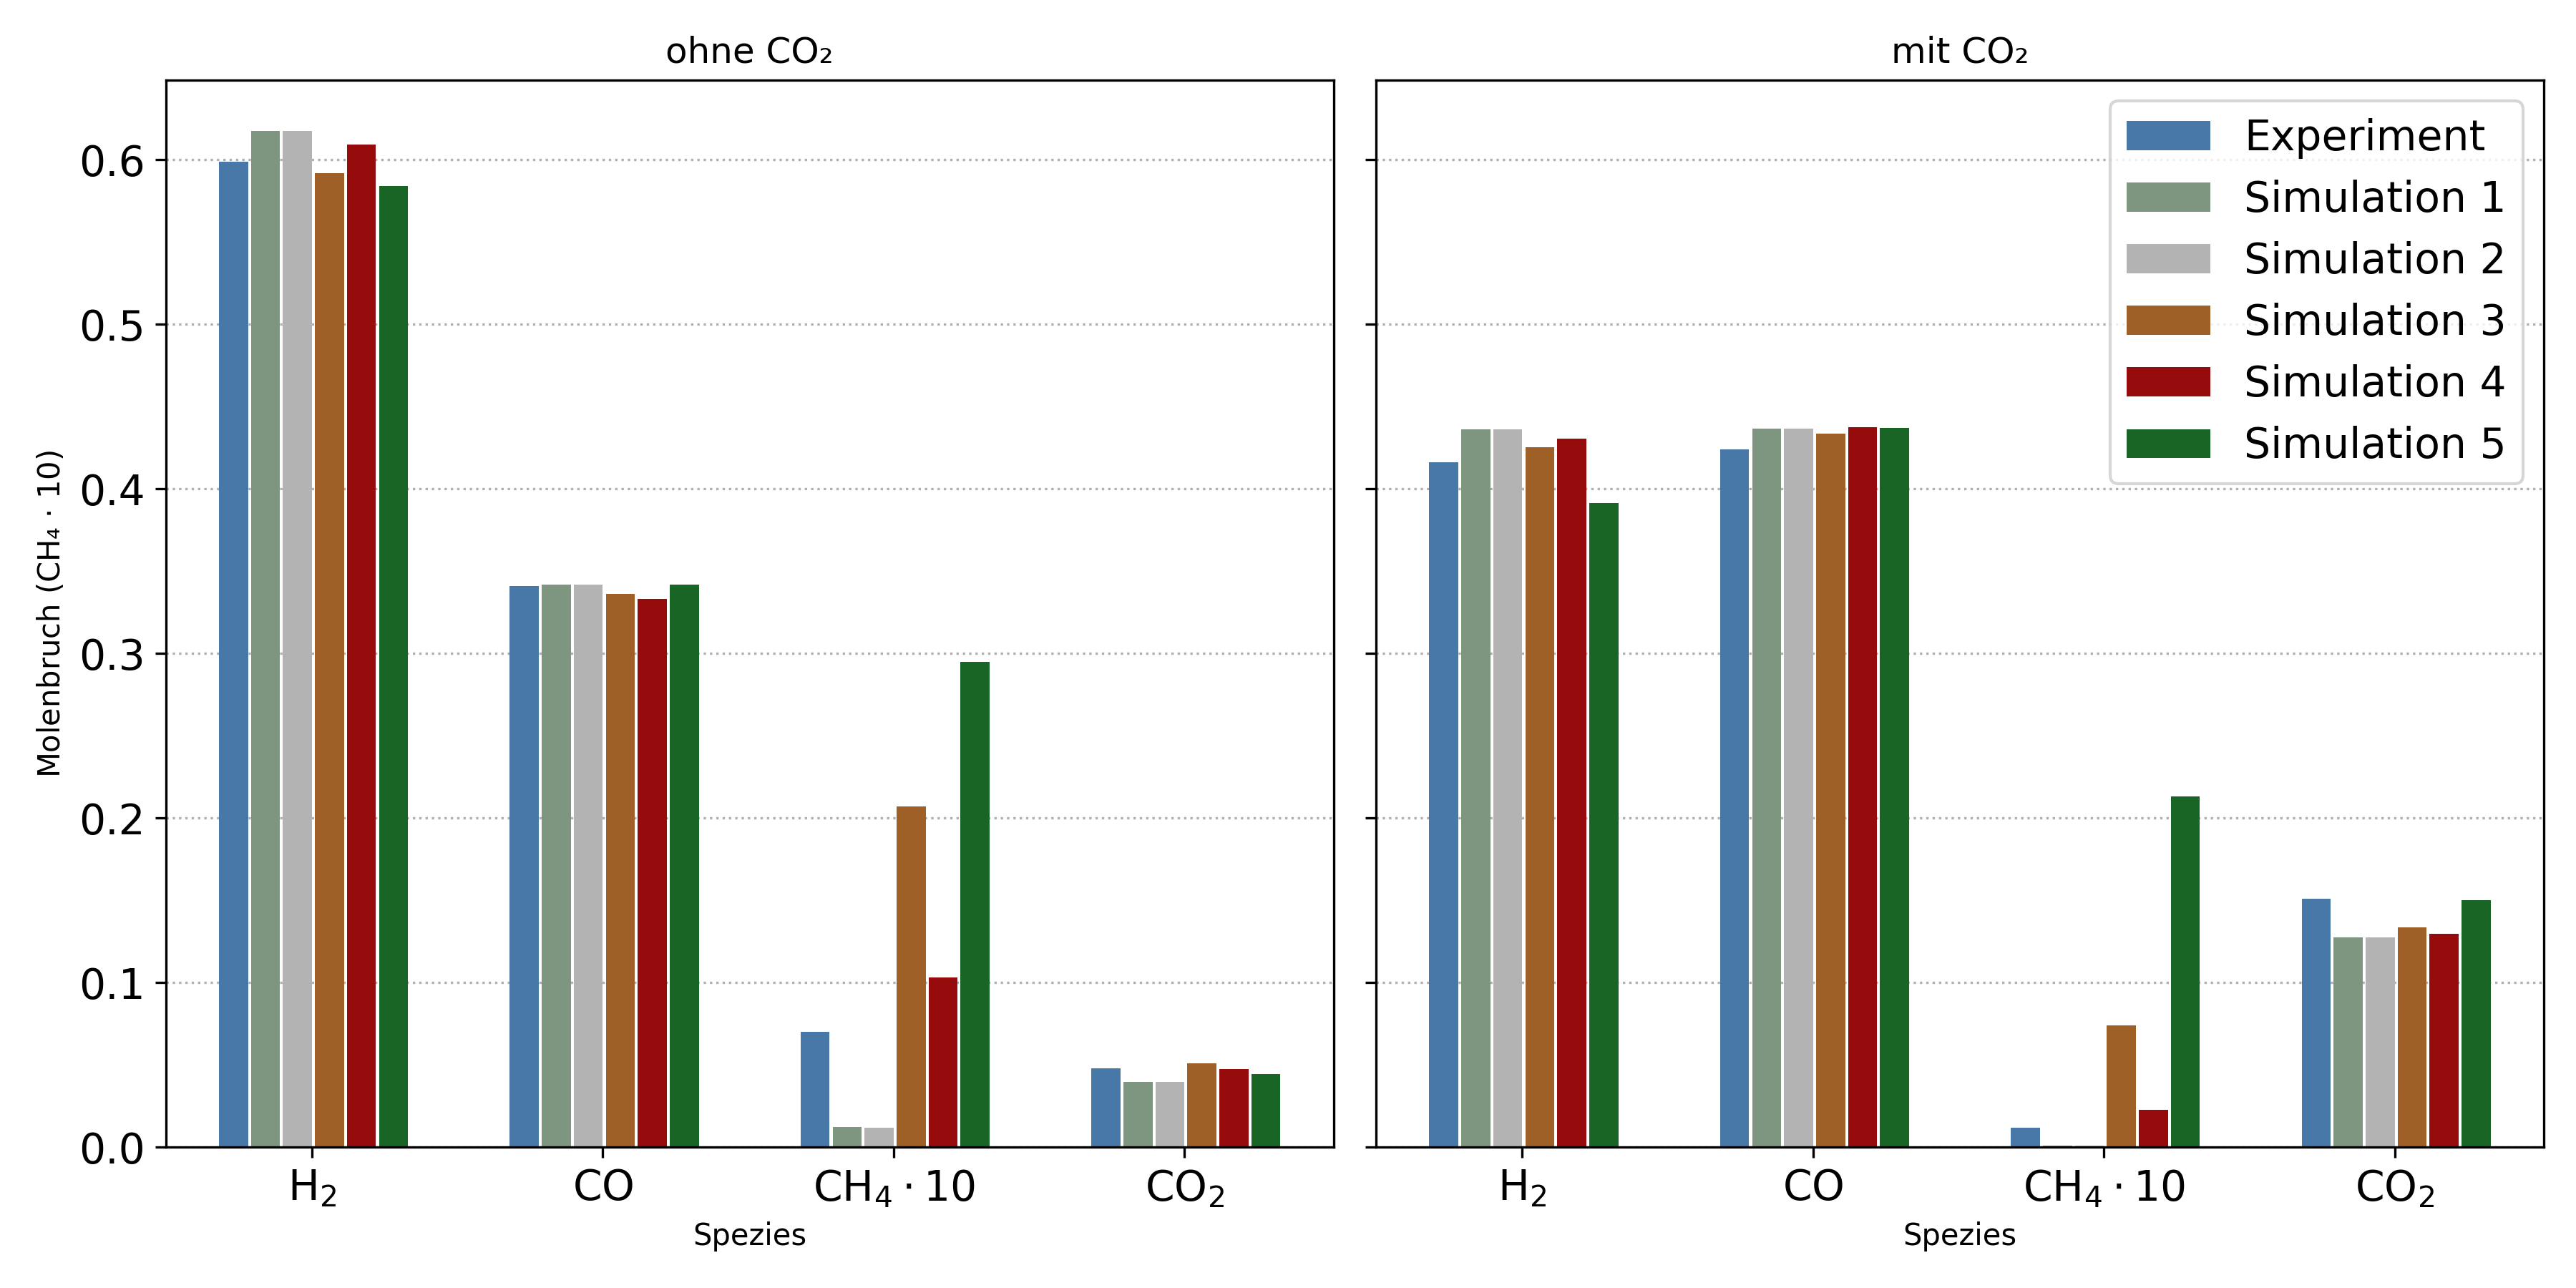
\includegraphics[width=0.9\linewidth]{img/Erweiterungen/Vergleich_Erweiterungen.png}
            \caption{Ergebnisse der Abgaszusammensetzungen und Vergleich mit den Werten der Experimente \cite{gonzales}}
            \label{fig:erweiterungen_vergleich_stoffe}
        \end{figure}
        Es ist erkennbar, dass die Größenordnungen aller Simulationen gleich sind. Dennoch gibt es Abweichungen zwischen den einzelnen Simulationen. Gerade der Schlupf von Methan (Methangehalt im Abgas) ist eine wichtige Kenngröße für diesen Prozess. Dabei kann man erkennen, dass die einfachsten Modelle einen deutlich zu niedrigen Methanschlupf haben, während die komplexen Modelle 3 und 5 einen deutlich zu hohen Schlupf von Methan aufweisen. Simulation 4 ist, wenn man nur den Schlupf von Methan betrachtet, die beste Simulation. 

        Zudem wurden in dem Reaktor durch zwei Thermoelemente Temperaturen gemessen, zusätzlich wurde die Austrittstemperatur als Vergleichswert bereits mit dem Programm AspenPlus bestimmt. Die Lage der Messpunkte in dem Reaktor sind in Abbildung \ref{fig:erweiterungen_messpunkte} zu erkennen. 
        \begin{figure}[H]
            \centering
            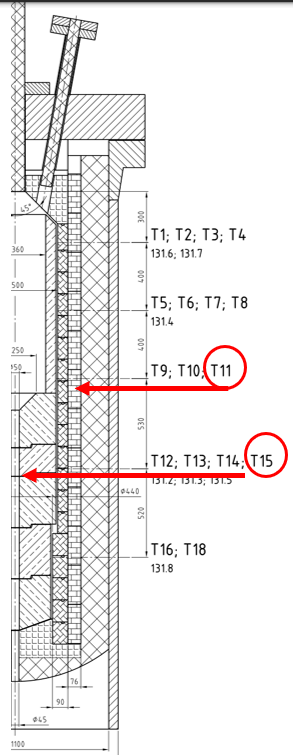
\includegraphics[width=0.2\linewidth]{img/Erweiterungen/Messpunkte.png}
            \caption{Messpunkte im Reaktor \cite{gonzales}}
            \label{fig:erweiterungen_messpunkte}
        \end{figure}
        Analog zu Abbildung \ref{fig:erweiterungen_vergleich_stoffe} können die Temperaturen an den verschiedenen Messpunkkten in Abbildung \ref{fig:erweiterungen_vergleich_temperaturen} dargestellt werden. 
        \begin{figure}[H]
            \centering
            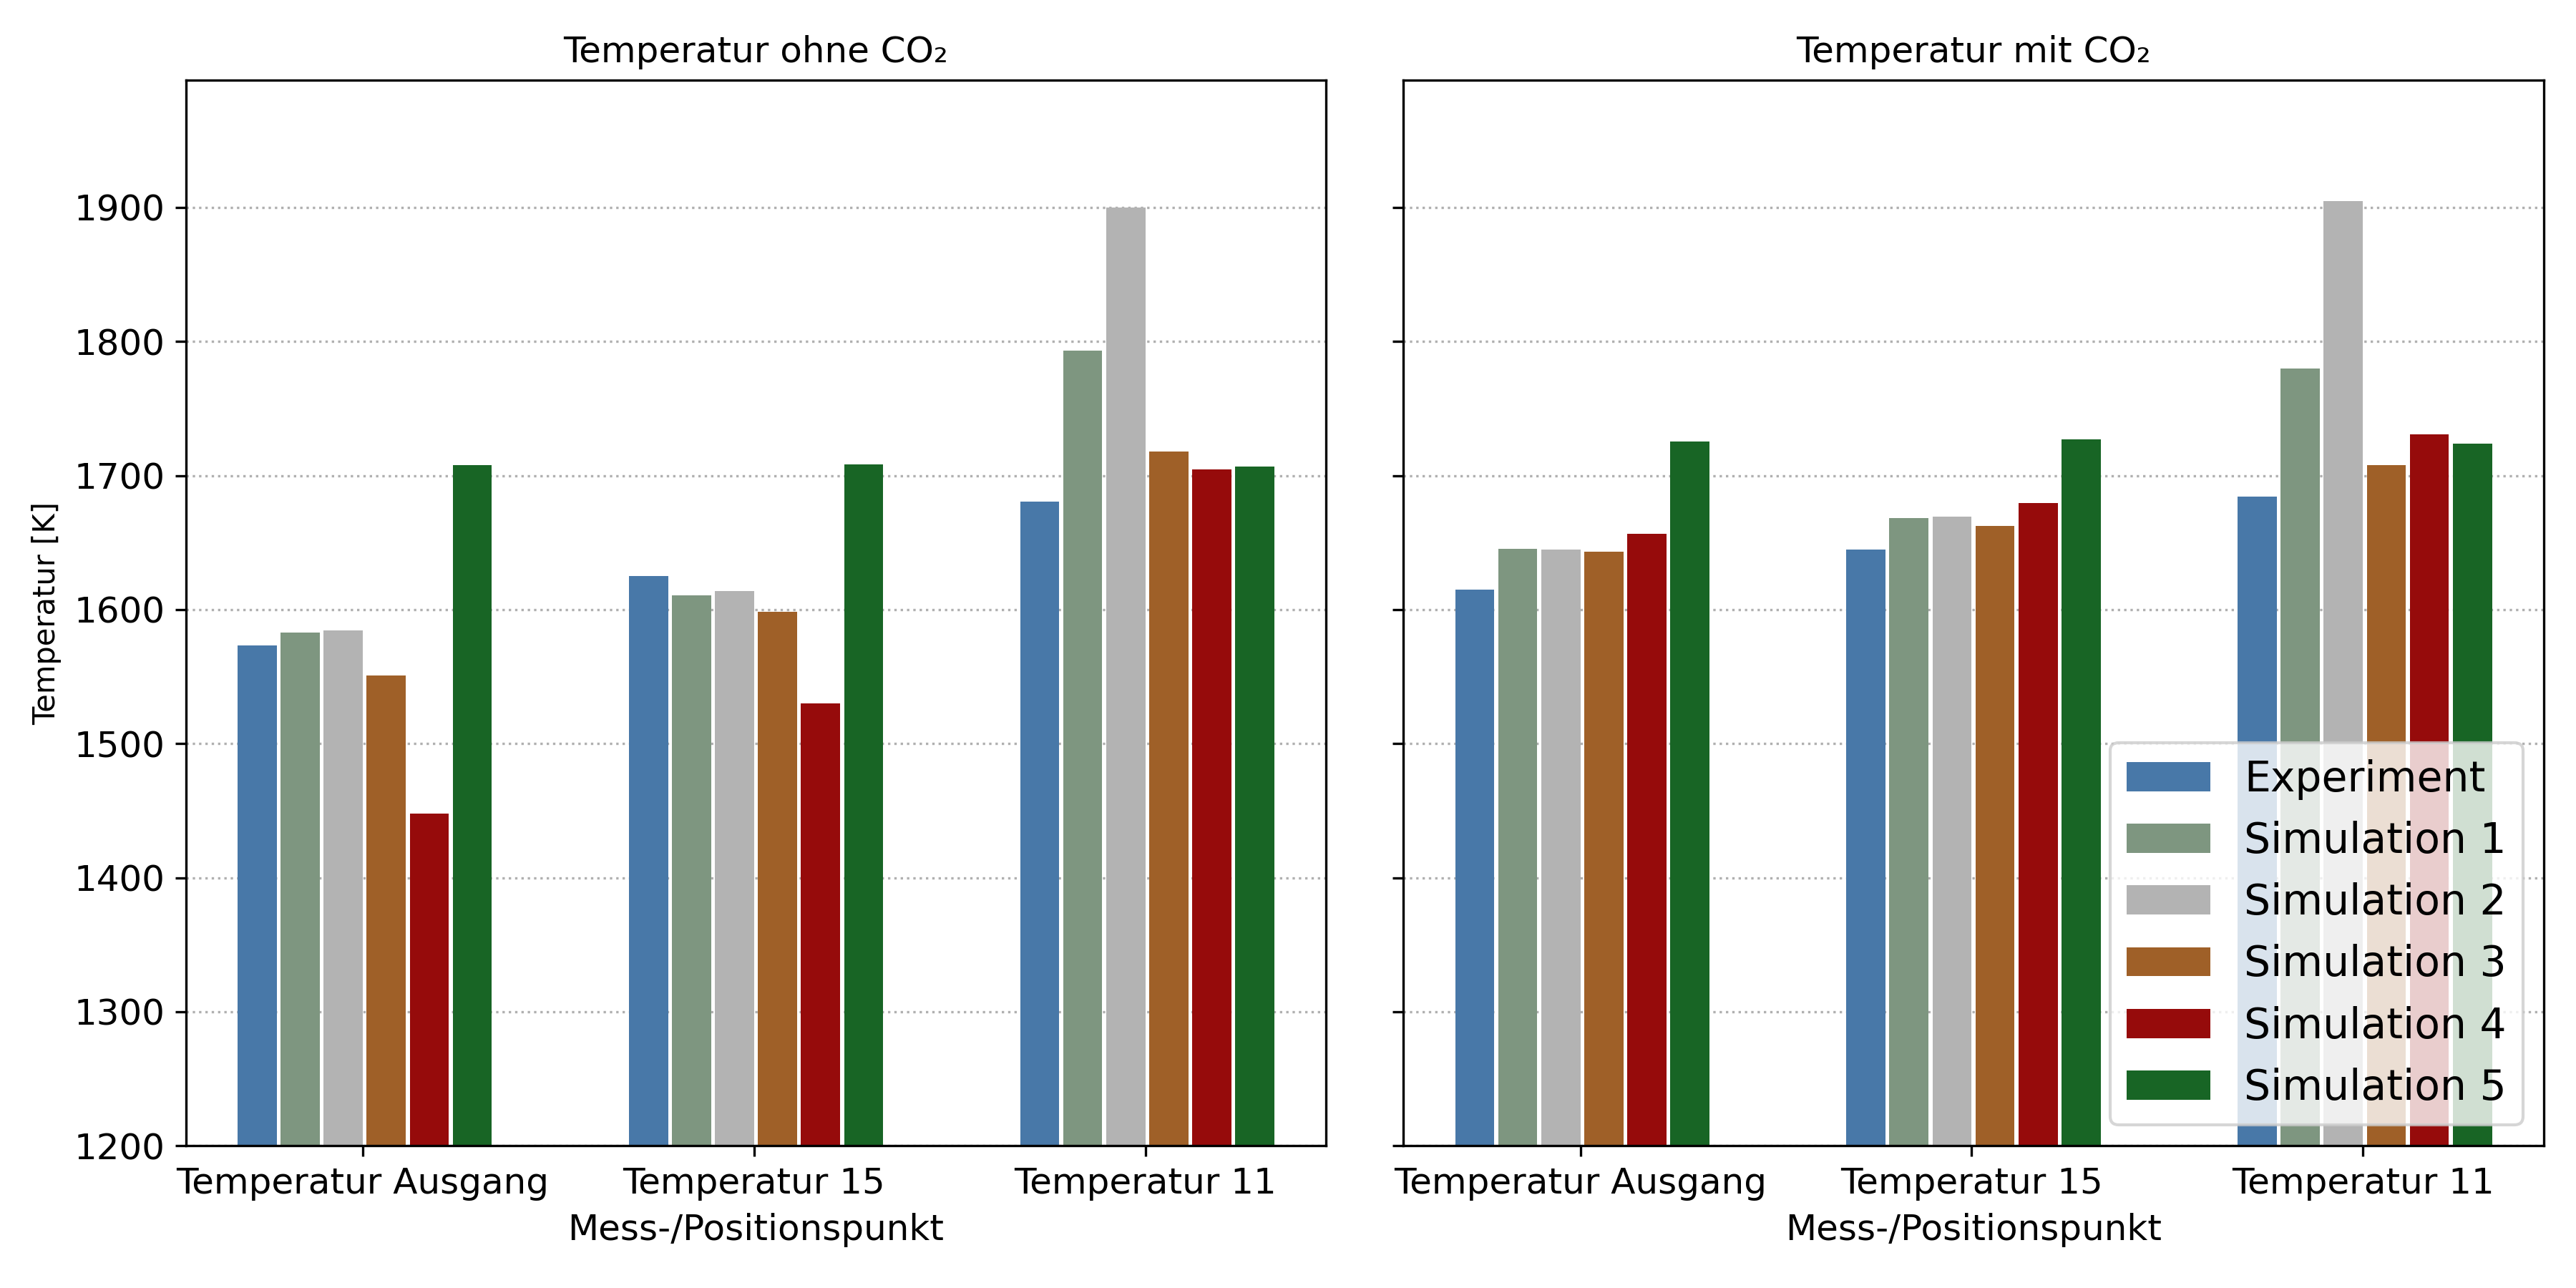
\includegraphics[width=0.9\linewidth]{img/Erweiterungen/Vergleich_Temperaturen.png}
            \caption{Ergebnisse der simulierten Temperaturen und Vergleich mit den gemessenen Temperaturen im Reaktor \cite{gonzales}}
            \label{fig:erweiterungen_vergleich_temperaturen}
        \end{figure}
        Wie auch bei den Stoffmengen liegen die Temperaturen größtenteils in einem ähnlichen Temperaturbereich. Es ist jedoch erkennbar, dass die Temperaturen der komplexesten Simulation allerdings deutlich zu hoch sind. Auch kann man eine deutlich zu geringe Temperatur des einfachsten Modells erkennen, die nur bei einer Zugabe von CO$_2$ auftritt, jedoch nicht ohne diese. 

        Zur quantitativen Bewertung der Modellgüte wurde ein relativer Fehlerwert eingesetzt. Für jede simulierte Größe wird der relative Fehler berechnet:
        \begin{align}
            E = \frac{\vert x_{sim} - x_{exp}\vert}{x_{exp}} 
        \end{align}
        Anschließend wird der Mittelwert über alle Größen gemittelt, sodass ein dimensionsloser Kennwert für jede Simulation entsteht. Dieser Wert ist direkt als mittlere prozentuale Abweichung intepretierbar, ein kleinerer Wert bedeutet eine höhere Übereinstimmung der Daten. 

        In Tabelle \ref{tab:relativer_fehler_vergleich} sind die Ergebnisse dieser Analyse aufgeführt. 
        \begin{table}[H]
            \centering
            \begin{tabular}{lcc}
                \toprule
                \textbf{Modell} & \textbf{Versuch 1} & \textbf{Versuch 2} \\
                \midrule
                1 & 0,159 & 0,261 \\
                2 & 0,169 & 0,190 \\
                3 & 0,300 & 0,765 \\
                4 & \textbf{0,096} & \textbf{0,167} \\
                5 & 0,494 & 2,426 \\
                \bottomrule
            \end{tabular}
            \caption{Bewertung der Modelle anhand des mittleren relativen Fehlers (MRE). Ein Wert von 0 entspricht perfekter Übereinstimmung, höhere Werte bedeuten größere Abweichungen.}
            \label{tab:relativer_fehler_vergleich}
        \end{table}
        In beiden Fällen weist Modell 4 die geringste Abweichung zu den experimentaldaten auf und kann somit als bestes Modell betrachtet werden. Im ersten Fall (ohne zusätzliches CO$_2$ im Feed) liegen alle Werte in einem moderatem Bereich, wobei insbesondere die einfachen Modelle 1 und 2 ebenfalls eine gute Genauigkeit vorweisen. 


        Im zweiten Fall (mit Zugabe von CO$_2$) verschlechtern sich alle Werte deutlich. Dies ist sowohl durch die erhöhte Komplexität der Reaktionschemie durch CO$_2$ (z.B. Dry Reforming und Wassergas-Shift-Reaktion) als auch auf die verstärkte Bedeutung kleiner Restkonzentrationen zurückzuführen, bei denen bereits kleine Mengen zu hohen relativen Fehlern führen. Besonders deutlich wird das am Modell 5, dessen MRE-Wert mehr als eine Größenordnung über den besten Modellen liegt.

        Auch ist in Modell 2 besonders auffällig, dass die Temperaturen deutlich unter allen anderen liegen. Dies kann nicht durch die nicht vorhandene Reaktion von Erdgas durch den Bypass erklärt werden, da dieses Modell ein viel zu geringen Schlupf von Methan aufweist. \alert{Vielmehr muss der Bypass ohne Rezirkulationszone zu einer Verschiebung der Gleichgewichtslagen in der Reformierungszone sorgen, wodurch die endothermen Reaktionen stark begünstigt werden.}

        Zusammenfassend lässt sich feststellen, dass die Modelle die Betriebsweisen ohne zusätzliches CO$_2$ als Feed besser modelliert werden können. Gleichzeitig bestätigt die Auswertung, dass ROM 4 in beiden Fällen die besten Ergebnisse liefert. 
\fi